%!TEX TS-program = pdflatex
\documentclass{beamer}
\usepackage{beamerthemeshadow}
\usepackage{lmodern}
\usepackage[beamer,customcolors]{hf-tikz}

\tikzset{hl/.style={
    set fill color=red!80!black!40,
    set border color=red!80!black,
  },
}
\usepackage[T1]{fontenc} 
\usepackage{fixltx2e}
\usepackage[brazil]{babel}
\usepackage{lmodern}
\usepackage[utf8]{inputenc}
\usepackage[english]{babel}
\usepackage{amsmath,amssymb,amsfonts,amsthm}
\usepackage[makeroom]{cancel}
\usepackage{graphicx}
\usepackage{wrapfig}
\usepackage{hyperref}
\usepackage{color}
\usepackage{colortbl}
\usepackage{xmpmulti}
\usepackage{multirow}
\usepackage{mdwtab}
\usepackage{verbatim}
\usepackage{textpos}

% tes
\usepackage{times}
\usepackage{tikz}
\usepackage{amsmath}
\usepackage{verbatim}
\usetikzlibrary{arrows,shapes}


\newcommand<>{\fullsizegraphic}[1]{
  \begin{textblock*}{0cm}(-1cm,-3.78cm)
  \includegraphics[width=\paperwidth]{#1}
  \end{textblock*}
}

%PACKAGE ADDED IN ORDER TO SHOW EXIT LOCATION SYMBOLS
\usepackage{pifont}
\usepackage{marvosym}
%IMPROVES WHITESPACING AROUND "..."
\usepackage{ellipsis}         
%ADDS THE 'SMILE FACE'
\usepackage{wasysym} 
%ADDS STRIKETHROUGH FONT
\usepackage{ulem}
\DeclareRobustCommand{\hsout}[1]{\texorpdfstring{\sout{#1}}{#1}}

\pdfpkresolution=2400

%USEFUL FOR HIGHLIGHTING TEXT AND CODE
\usepackage{tikz}
\usetikzlibrary{positioning,calc,arrows,shapes,shadows,trees}
\tikzset{onslide/.code args={<#1>#2}{%
  \only<#1>{\pgfkeysalso{#2}} % \pgfkeysalso doesn't change the path
}}
\usepackage{smartdiagram}

\usepackage{microtype}


\title{Uma abordagem para criação, reúso e aplicação de refatorações no contexto da modernização dirigida a arquitetura}

\date{}

\author{Rafael Serapilha Durelli\\Orientador: Prof. Dr. Márcio Eduardo Delamaro\\Colaborador: Prof. Dr. Valter Vieira de Camargo\\}

\titlegraphic{
\includegraphics[width=0.55\textwidth]{figures/figuraLocais.pdf}} %,height=0.12\textheight
\makeindex

\newcommand{\nl}{\ \par \noindent }
\newcommand{\hl}[1]{\textbf{#1}}
\newcommand{\hll}[1]{\underline{#1}}

\usetheme{Warsaw}
% \titlegraphic{\scalebox{0.125}{\includegraphics{fapesp_logo.pdf}}}

%PRESENTATION
\begin{document} 

\tikzstyle{every picture}+=[remember picture]

% By default all math in TikZ nodes are set in inline mode. Change this to
% displaystyle so that we don't get small fractions.
\everymath{\displaystyle}

%SHOW SLIDE NUMBER
\setbeamertemplate{footline}[frame number]

%PRESENTATION TITLE
\frame[label=firstslide]{\maketitle}


\begin{frame}{Agenda}
\tableofcontents
\end{frame}


\section{Introdução}
\label{sec:introducao}

\subsection{Contextualização, Motivações, Objetivos e Sínteses da Pesquisa Conduzida}

%\subsection{Objetivos e Sínteses da Pesquisa Conduzida}

\begin{frame}\frametitle{Introdução - Contextualização}

\begin{itemize}
    \item Sistemas Legados;
        \begin{itemize}
            \item Documentação inconsistente;
            \item Manutenção comprometida;
            \item Tarefa não trivial e propensa a erros.
        \end{itemize}
    \item OMG lançou em 2003 a ADM;
        \begin{itemize}
            \item Padronizar processos de reengenharia;
            \item Utilizando metamodelos padronizados.
        \end{itemize}
    \item KDM;
        \begin{itemize}
            \item Diversas metaclasses (código-fonte, arquitetura, arquitetura);
        \end{itemize}
\end{itemize}


\begin{itemize}
    \begin{minipage}[b]{9.8cm} \item Sistemas Legados; 
    \vspace{.2cm}
        \begin{itemize}
            \begin{minipage}[b]{9.8cm} \item Documentação inconsistentes; 
            \vspace{.2cm}
            \end{minipage}
            \begin{minipage}[b]{9.8cm} \item Dificulta sua manutenção; 
            \vspace{.2cm}
            \end{minipage}
            \begin{minipage}[b]{9.8cm} \item Substituí-lo é uma tarefa muito cara e propensa a erros. 
            \vspace{.2cm}
            \end{minipage}
        \end{itemize}
    \end{minipage}
    \begin{minipage}[b]{9.8cm} \item OMG lançou em 2003 a ADM; 
    \vspace{.2cm}
        \begin{itemize}
            \begin{minipage}[b]{9.8cm} \item Documentação inconsistentes; 
            \vspace{.2cm}
            \end{minipage}
            \begin{minipage}[b]{9.8cm} \item Dificulta sua manutenção; 
            \vspace{.2cm}
            \end{minipage}
            \begin{minipage}[b]{9.8cm} \item Substituí-lo é uma tarefa muito cara e propensa a erros. 
            \vspace{.2cm}
            \end{minipage}
        \end{itemize}
    \end{minipage}
\end{itemize}

\end{frame}

\begin{frame}\frametitle{Introdução - Contextualização}

\begin{block}{\textit{Architecture-Driven Modernization} (ADM)}
\begin{minipage}[b]{10.80cm}
OMG definiu a ADM cujo objetivo principal é padronizar processos de reengenharia por meio de metamodelos padronizados~\cite{KDM:specification,KDM:ISO}.
\end{minipage}  
\end{block}

\begin{block}{\textit{Knowledge Discovery Metamodel} (KDM)}
\begin{minipage}[b]{10.80cm}
Knowledge Discovery Metamodel (KDM) é o principal metamodelo da ADM. E possui uma ampla quantidade de metaclasses para representar diferentes níveis de abstração.
\end{minipage}  
\end{block}

\begin{itemize}
    \begin{minipage}[b]{9.8cm} \item Código-fonte; 
    \vspace{.2cm}
    \end{minipage}
    \begin{minipage}[b]{9.8cm} \item Arquitetura, regras de negócio e outros conceitos abstratos do sistema; 
    \vspace{.2cm}
    \end{minipage}
    \begin{minipage}[b]{9.8cm} \item GUI, arquivos de configuração, bases de dados, etc; 
    \vspace{.2cm}
    \end{minipage}
\end{itemize}

\end{frame}

\begin{frame}\frametitle{Introdução - Contextualização}

\begin{block}{\textit{Architecture-Driven Modernization} (ADM)}
\begin{minipage}[b]{10.80cm}
A ADM almeja que a comunidade comece a desenvolver algoritmos e técnicas que sejam dependentes e específicas apenas do metamodelo KDM, e não de plataformas, metamodelos proprietários ou linguagens de programação específicas.
\end{minipage}  
\end{block}

Por exemplo: \vspace{.35cm}

\begin{itemize}
  \begin{minipage}[b]{9.8cm}  
  \item  Algoritmos de refatorações~\cite{durelli_catalogo} específicos para o KDM.
  \vspace{.4cm}\end{minipage}
  \begin{minipage}[b]{9.8cm} 
  \item  Algoritmos de mineração de interesses transversais, utilizando como base o metamodelo KDM~\cite{Durelli:2013_ACM, dani_san, daniel_san_journal}.
  \vspace{.4cm}\end{minipage}
\end{itemize}

\end{frame}

\begin{frame}\frametitle{Introdução - Contextualização}

\begin{block}{\textit{Knowledge Discovery Metamodel} (KDM)}
\begin{minipage}[b]{10.80cm}
Metamodelo padrão de representação de sistemas  dentro das ferramentas de modernização baseadas em ADM. Entretanto, muitas ferramentas utilizarão o metamodelo UML para a apresentação gráfica do sistema.
\end{minipage}  
\end{block}

KDM permite: \vspace{.35cm}

\begin{itemize}
  \begin{minipage}[b]{9.8cm}  
  \item Algoritmos possam ser importados/exportados entre ferramentas de modernização;
  \vspace{.4cm}\end{minipage}
  \begin{minipage}[b]{9.8cm} 
  \item  Propiciando interoperabilidade e consequentemente melhorando a produtividade dos desenvolvedores/mantenedores.
  \vspace{.4cm}\end{minipage}
\end{itemize}

\end{frame}

\begin{frame}\frametitle{Introdução - Contextualização}

\begin{block}{\textit{Architecture-Driven Modernization} (ADM)}
\begin{minipage}[b]{10.80cm}
Um processo de modernização típico da ADM possui três principais passos: (\textit{i}) engenharia reversa; (\textit{ii}) reestruturação; e (\textit{iii}) engenharia avante.
\end{minipage}  
\end{block}

\begin{block}{Refatorações}
\begin{minipage}[b]{10.80cm}
Considerando o processo de modernização da ADM, uma atividade fundamental durante o passo de reestruturação são as refatorações.
\end{minipage}  
\end{block}


\end{frame}

\begin{frame}\frametitle{Introdução - Contextualização}

\begin{block}{Refatorações}
\begin{minipage}[b]{10.80cm}
Embora o conceito de refatoração seja bem conhecido e aplicado em código-fonte, sua aplicação em modelos ainda apresentada desafios de pesquisa~\cite{Gorp}.
\end{minipage}  
\end{block}

Refatorações em modelos:

\begin{itemize}
  \begin{minipage}[b]{9.8cm}  
  \item + complexas do que refatorações ``tradicionais'';
  \vspace{.4cm}\end{minipage}
  \begin{minipage}[b]{9.8cm} 
  \item  Não possuem características específicas de linguagens de programação;
  \vspace{.4cm}\end{minipage}
  \begin{minipage}[b]{9.8cm} 
  \item  A maior parte das pesquisas aplicam de refatorações na UML~\cite{Salem_2008, revisao_sistematica_uml_refactoring}.
  \vspace{.4cm}\end{minipage}
\end{itemize}


\end{frame}

\begin{frame}\frametitle{Introdução - Contextualização}

\begin{block}{Cenário Ideal}
\begin{minipage}[b]{10.80cm}
\begin{itemize}
  \item Aplicar refatorações em diagramas da UML;
  \item Internamente aplicar em instâncias do KDM;
  \item Artefatos podem continuar consistentes e sincronizados;
  \item Algoritmos de refatorações podem ser reutilizados em diversas ferramentas de modernização,
\end{itemize}
\end{minipage}  
\end{block}

Assim, vislumbrou-se uma oportunidade de conduzir essa pesquisa no contexto da ADM. 

\end{frame}

\begin{frame}\frametitle{Introdução - Motivações}


\begin{block}{Motivações}
\begin{minipage}[b]{10.80cm}
As princípais motivações que levaram ao desenvolvimento desta tese foram:
\end{minipage}  
\end{block}

\begin{enumerate}
	\begin{minipage}[b]{9.5cm}\item Carência de ferramentas de modernização que permitem aplicar refatorações em diagramas UML que são representações gráficas de modelos KDM.\\\end{minipage}\\
	\begin{minipage}[b]{9.5cm}\item Escassez de abordagens de criação de refatorações para o KDM.\\\end{minipage}\\		
	\begin{minipage}[b]{9.5cm}\item Ausência de um metamodelo que forneça uma terminologia comum, padronizada e independente de linguagem para a especificação de refatorações.\end{minipage}\\		
\end{enumerate}


\end{frame}

\begin{frame}\frametitle{Introdução - Objetivos}


\begin{block}{Objetivos}
\begin{minipage}[b]{10.80cm}
O objetivo é apresentar uma abordagem para criação e disponibilização de refatorações para o metamodelo KDM e uma apoio ferramental que permite aplicá-las em diagramas de classe da UML. 
\end{minipage}  
\end{block}

\begin{enumerate}
	\begin{minipage}[b]{9.5cm}\item Tornar a criação de refatorações para o metamodelo KDM um processo sistemático e guiado.\\\end{minipage}\\
	\begin{minipage}[b]{9.5cm}\item Potencializar o reúso das refatorações desenvolvidas.\\\end{minipage}\\		
	\begin{minipage}[b]{9.5cm}\item Viabilizar a aplicação de refatorações em modelos KDM a partir de diagramas UML.\end{minipage}\\		
\end{enumerate}


\end{frame}



%\begin{frame}
 % \fullsizegraphic{figures/NovaFiguraSintexeAbordagem.pdf}
%\end{frame}

\begin{frame}\frametitle{Introdução - Síntese da Pesquisa Conduzida}

\begin{figure}[h]
	\centering
	\label{fig:abordagem_kdm_tese_processo}
	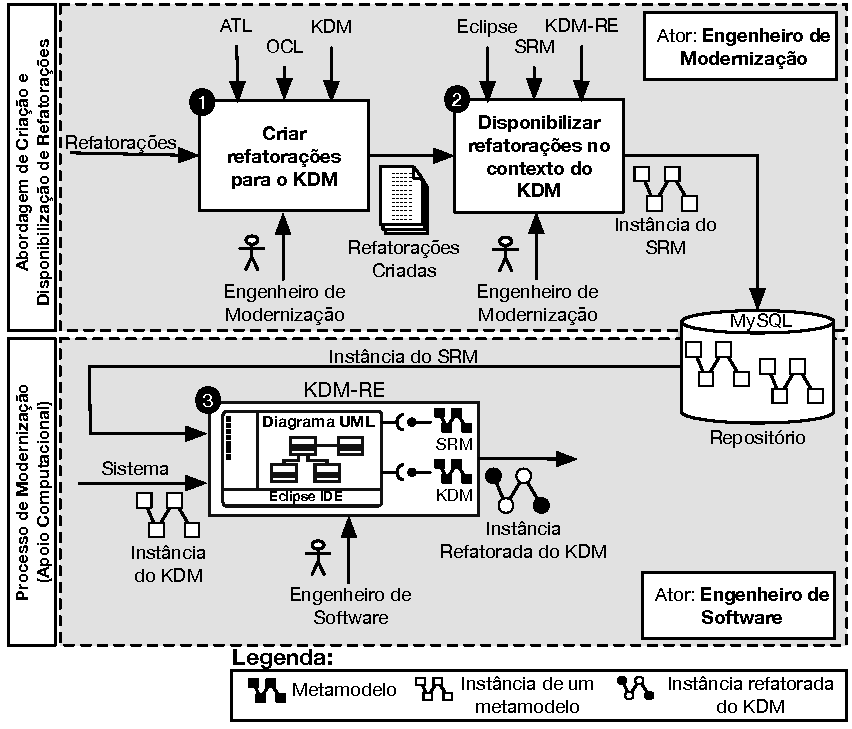
\includegraphics[scale=0.45]{figures/NovaFiguraSintexeAbordagem.pdf}
\end{figure}

\end{frame}


\section{Fundamentação Teórica}
%\subsection{Engenharia Dirigida por Modelos e Refatorações}
\label{sub:goal}
\subsection{Refatorações}

\begin{frame} \frametitle{Fundamentação Teórica - Refatorações}

\begin{block}{Refatorações}
\begin{minipage}[b]{10.80cm}
São transformações que reestruturam um determinado sistema com o objetivo de melhorar o \textit{design}, a evolução e o reúso de sistemas desenvolvidos no paradigma orientado a objeto\cite{OPDYKE_1992}.
\end{minipage}  
\end{block}

\vspace{0.2cm}
\indent Refatoração ajuda a tornar o código mais legível e também tem como objetivo solucionar problemas de códigos mal escritos~\cite{Chikofsky_cross};\\
\vspace{0.2cm}
\indent Refatoração não inclui nenhuma mudança no sistema, isto é, refatoração não deve adicionar novas funcionalidades ao sistema; \\
\vspace{0.2cm}
\end{frame}

\begin{frame}[t]\frametitle{Fundamentação Teórica - Refatorações}


Opdyke~\cite{OPDYKE_1992}, onde o autor definiu 26 refatorações de baixa granularidade. O catálogo mais completo e extensivo de refatorações foi definido por Fowler~\cite{Fowler1999}.

\vspace{.3cm}

\begin{columns}
  \begin{column}{0.5\textwidth}
\tikz[baseline]{
            \node[fill=blue!20,anchor=base] (t1)
            {
            
            \begin{minipage}[b]{7cm} 
            \structure{\ding{202}} Criar um membro; 
            \newline
            \structure{\ding{203}} Deletar um membro;
            \newline
            \structure{\ding{204}} Renomear um membro; 
            \newline
            \structure{\ding{205}} Mover um membro. 
            \end{minipage}
              
            % \end{itemize}
            };
        }

        \tikz[baseline]{
            \node[fill=red!20,anchor=base] (t2)
            {
            
            \begin{minipage}[b]{7cm} 
            \structure{\ding{206}} \textit{Composing Methods}; 
            \newline
            \structure{\ding{207}} \textit{Moving Features Between Objects};
            \newline
            \structure{\ding{208}} \textit{Dealing with Generalization}, etc.
            \end{minipage}
            };
        }
  \end{column}
  \begin{column}{0.5\textwidth} 
      \flushright
    % \begin{description}
      % \item Fine \color{white}~~~~~~~~~~~~~    
      \tikz\node [fill=blue!20,draw,circle] (n1) {Opdyke};
    % \end{description}
    % \begin{description}
      % \item \small Way too complex \color{white}\normalsize  
      \tikz\node [fill=red!20, below of=n1, draw,circle] (n2) {Fowler};
    % \end{description}
  \end{column}
\end{columns}

\end{frame}

\begin{frame} \frametitle{Fundamentação Teórica - Transformações e Refatorações de Modelos}

\begin{block}{Refatorações de Modelos}
\begin{minipage}[b]{10.80cm}
São transformação de modelos\footnote{Transformação e Refatoração de modelos são utilizadas nesta tese de forma intercambiáveis.} que têm como principal objetivo melhorar a estrutura do modelo e também preservar suas características internas.
\end{minipage}  
\end{block}

\begin{itemize}
  \item Vertical ou horizontal;
	\item Endógenas ou exógenas;
	\item Bidirecionais. 
\end{itemize}

\end{frame}

\begin{frame} \frametitle{Fundamentação Teórica - Transformações e Refatorações de Modelos}

\begin{figure}[h]
	\centering
%	\caption{Transformações Endógenas.}
	\label{fig:abordagem_kdm_tese_processo}
	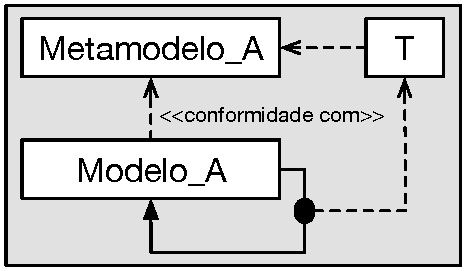
\includegraphics[scale=0.65]{figures/transformacaoModeloB.pdf}
\end{figure}

\begin{block}{Endógenas ou exógenas}
\begin{minipage}[b]{10.80cm}
Endógenas, os modelos envolvidos são expressos na mesma linguagem de modelagem. Nas transformações exógenas, os modelos que participam da transformação são de linguagens diferentes.
\end{minipage}  
\end{block}


\end{frame}

\subsection{Modernização Dirigida a Arquitetura - ADM}

\begin{frame}[fragile]\frametitle{Modernização Dirigida a Arquitetura - ADM}

\begin{block}{\textbf{ADM}}
\begin{minipage}[b]{10.80cm}
OMG lançou em 2003 o termo Modernização Dirigida a Arquitetura (do inglês - \textit{Architecture-Driven Modernization} (ADM) cujo objetivo principal é padronizar processos de reengenharia por meio de metamodelos padronizados~\cite{ADM:OMG}.
\end{minipage}  
\end{block}


\begin{itemize}
  \item Estabelecer metamodelos padronizados para auxiliar todo o  processo da reengenharia de software;
  \item ADM não objetiva substituir o processo tradicional da reengenharia de software.
\end{itemize}


\end{frame}

\begin{frame}[fragile]\frametitle{Modernização Dirigida a Arquitetura - ADM}

\begin{table}[h]
\centering
\scriptsize
\caption{Estado atual dos metamodelos da ADM.}
\label{tab:todos_os_meta_modelos_da_ADM}
\begin{tabular}{|l|l|l|l|}
\hline
\multicolumn{1}{|c|}{Metamodelo}                                         & \multicolumn{1}{c|}{Situação}           & \multicolumn{1}{c|}{Versão} & \multicolumn{1}{c|}{Data}          \\ \hline
\textit{ADM Pattern Recognition} (ADMPR)                     & Em desenvolvimento &\multicolumn{1}{c|}{\textemdash}&\multicolumn{1}{c|}{\textemdash}\\ \hline
\textit{ADM Refactoring Specification} (ADMRS)               & Em desenvolvimento &\multicolumn{1}{c|}{\textemdash}&\multicolumn{1}{c|}{\textemdash}\\ \hline
\textit{ADM Visualization Specification} (ADMVS)             & Em desenvolvimento &\multicolumn{1}{c|}{\textemdash}&\multicolumn{1}{c|}{\textemdash}\\ \hline
\sigla{ASTM}{\textit{Abstract Syntax Tree Metamodel}}               & \multicolumn{1}{c|}{Disponível}         & \multicolumn{1}{c|}{1.0}    & \multicolumn{1}{c|}{2011}  \\ \hline
\textit{Knowledge Discovery Metamodel} (KDM)                 & \multicolumn{1}{c|}{Disponível}         & \multicolumn{1}{c|}{1.3}    & \multicolumn{1}{c|}{2011}   \\ \hline
\multirow{2}{*}{\textit{Structured Metrics Metamodel} (SMM)} & \multicolumn{1}{c|}{Disponível}         & \multicolumn{1}{c|}{1.0}    & \multicolumn{1}{c|}{2012}  \\ \cline{2-4} 
                                                    & Em desenvolvimento & \multicolumn{1}{c|}{1.1}    & \multicolumn{1}{c|}{2013} \\ \hline
\end{tabular}
\end{table}

\end{frame}

\begin{frame}[fragile]\frametitle{Modernização Dirigida a Arquitetura - ADM}

\begin{figure}[h]
	\centering
	\label{fig:abordagem_kdm_tese_processo}
	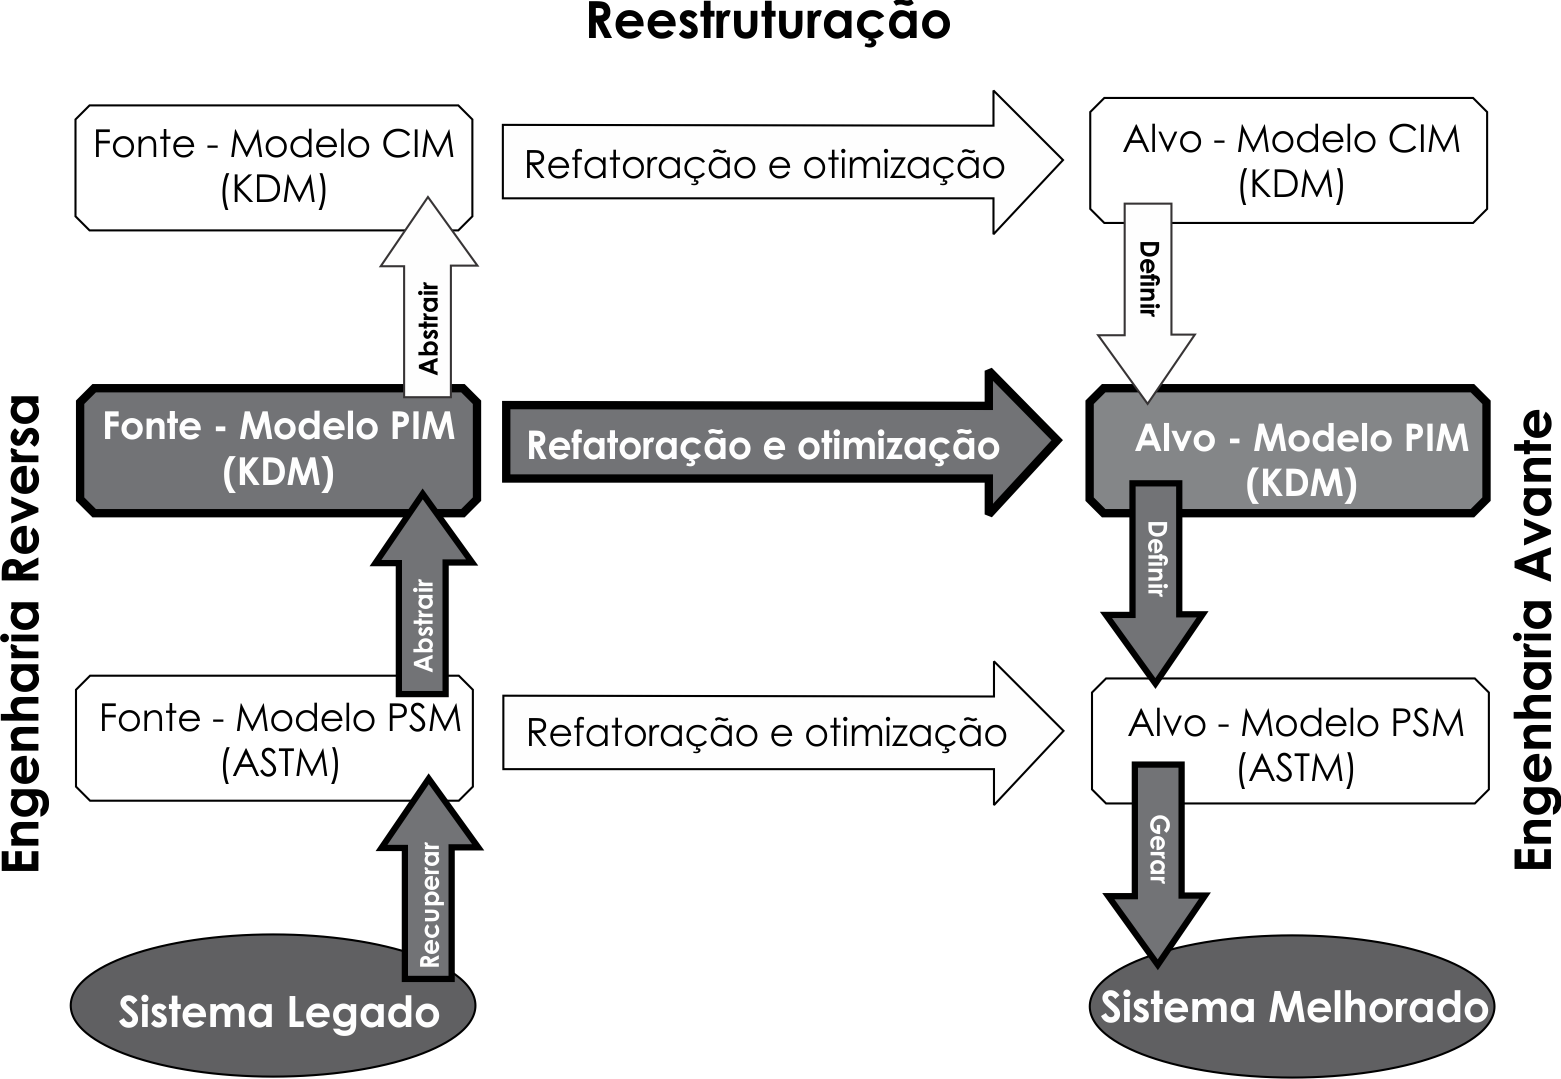
\includegraphics[scale=0.65]{figures/modelo-ferradura.png}
\end{figure}


\end{frame}


\begin{frame}[fragile]\frametitle{Knowledge Discovery Metamodel - KDM}

\begin{block}{\textbf{Knowledge Discovery Metamodel}}
\begin{minipage}[b]{10.80cm}
 KDM é um metamodelo que representa existentes artefatos de software, seus elementos, associações e ambientes operacionais.
\end{minipage}  
\end{block}


\begin{figure}[h]
	\centering
	\label{fig:abordagem_kdm_tese_processo}
	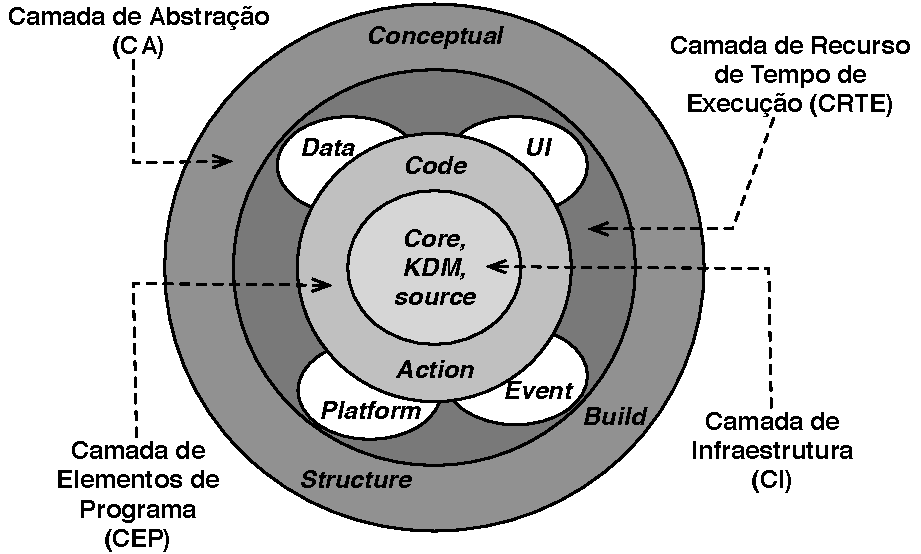
\includegraphics[scale=0.45]{figures/kdm_layers.pdf}
\end{figure}


\end{frame}


\begin{frame}[fragile]\frametitle{Knowledge Discovery Metamodel - KDM}

Algumas metaclasses do KDM.

\begin{columns}
    \begin{column}{0.48\textwidth}
        \begin{figure}[h]
	\centering
	\label{fig:abordagem_kdm_tese_processo}
	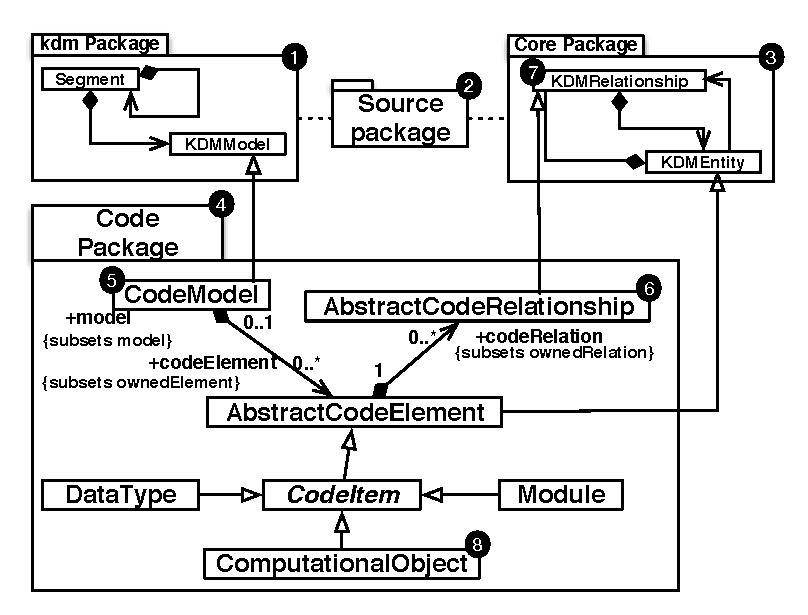
\includegraphics[scale=0.45]{figures/codeModel.pdf}
\end{figure}
    \end{column}
    \begin{column}{0.48\textwidth}
        \begin{figure}[h]
	\centering
	\label{fig:abordagem_kdm_tese_processo}
	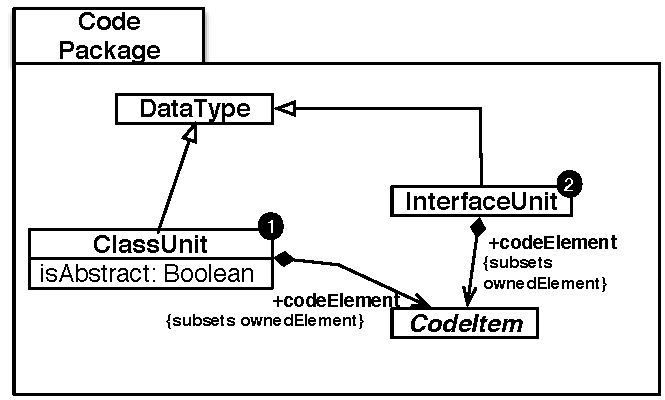
\includegraphics[scale=0.45]{figures/ClassUnit_InterfaceUnit.pdf}
\end{figure}
    \end{column}
\end{columns}

\end{frame}

\begin{frame}[fragile]\frametitle{Knowledge Discovery Metamodel - KDM}

 Algumas metaclasses do KDM.

\begin{columns}
    \begin{column}{0.48\textwidth}
        \begin{figure}[h]
	\centering
	\label{fig:abordagem_kdm_tese_processo}
	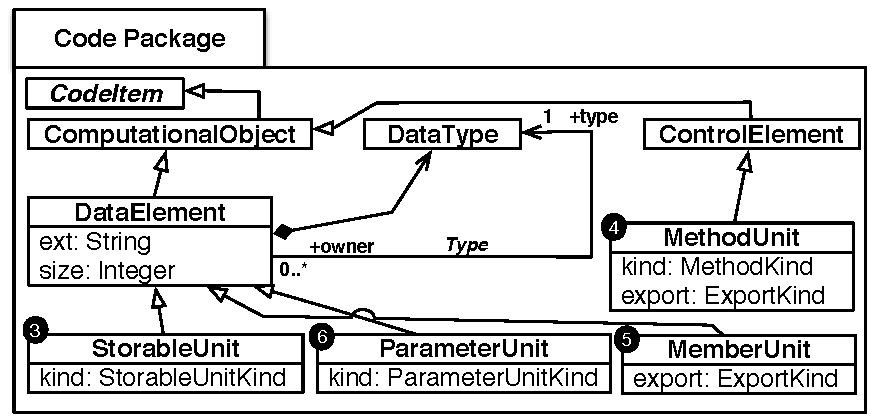
\includegraphics[scale=0.40]{figures/StorableUnit_MethodUnit2.pdf}
\end{figure}
    \end{column}
    \begin{column}{0.48\textwidth}
        \begin{table}[h]
\centering
\scriptsize
%\caption{Metaclasses para modelagem de estruturas estáticas do código-fonte.}
\label{tab:meta_classes_pacoteCODE}
\begin{tabular}{|l|l|}
\hline
Código-Fonte & Metaclasses do KDM \\ \hline
\multicolumn{1}{|c|}{Classe}                   & \multicolumn{1}{|c|}{\texttt{ClassUnit}}           \\ \hline
\multicolumn{1}{|c|}{Interface}                & \multicolumn{1}{|c|}{\texttt{InterfaceUnit}}       \\ \hline
\multicolumn{1}{|c|}{Método}                   & \multicolumn{1}{|c|}{\texttt{MethodUnit}}          \\ \hline
\multicolumn{1}{|c|}{Atributo}                 & \multicolumn{1}{|c|}{\texttt{StorableUnit}}        \\ \hline
\multicolumn{1}{|c|}{Variável Local}           & \multicolumn{1}{|c|}{\texttt{MemberUnit}}          \\ \hline
\multicolumn{1}{|c|}{Parâmetro}                & \multicolumn{1}{|c|}{\texttt{ParameterUnit}}       \\ \hline
\multicolumn{1}{|c|}{Associação}               & \multicolumn{1}{|c|}{\texttt{KDMRelationShip}}     \\ \hline
\end{tabular}
\end{table}
    \end{column}
\end{columns}

\end{frame}


\begin{frame}[fragile]\frametitle{Knowledge Discovery Metamodel - KDM}

\begin{block}{\textbf{Knowledge Discovery Metamodel}}
\begin{minipage}[b]{10.80cm}
 KDM possui outras metaclasses para representar diversos níveis de abstração:
\end{minipage}  
\end{block}

\begin{itemize}
  \item Pacote \textit{Action}: \textit{Calls}, \textit{Creates}, \textit{Writes}, etc;
  \item Pacote \textit{Structure}: \textit{Layer}, \textit{ArchitectureView}, \textit{SoftwareSystem}, \textit{Component}, etc;
  \item Pacote \textit{Data}: \textit{RelationalTable}, \textit{ColumnSet}, \textit{UniqueKey}, etc;
\end{itemize}

\end{frame}


%\subsection{Modernização dirigida a arquitetura (ADM) e Knowledge Discovery Metamodel (KDM)} % (fold)


\section{Uma abordagem para criar refatorações para o KDM}

\begin{frame}
\frametitle{Uma abordagem para criar refatorações para o KDM}

\begin{minipage}{10.8cm}
    Abordagem criada para guiar o engenheiro de modernização durante a criação de refatorações para o KDM (DURELLI et al., 2014a)
\end{minipage}  

\begin{block}{\textbf{Refatoração no contexto da Tese}}
\begin{minipage}[b]{10.80cm}
 Uma refatoração é uma tripla ordenada \textbf{R}:
\end{minipage}  
\end{block}



\tikzstyle{na} = [baseline=-.5ex]

\begin{itemize}[<+-| alert@+>]
    \item Pré-condição (OCL)
        \tikz[na] \node[coordinate] (n1) {};
\end{itemize}

% Below we mix an ordinary equation with TikZ nodes. Note that we have to
% adjust the baseline of the nodes to get proper alignment with the rest of
% the equation.
\begin{equation*}
R = (\tikz[baseline]{
            \node[fill=blue!20,anchor=base] (t1)
            {pre};
        } +
        \tikz[baseline]{
            \node[fill=red!20, ellipse,anchor=base] (t2)
            {T};
        } +
        \tikz[baseline]{
            \node[fill=green!20,anchor=base] (t3)
            {pos};
        })
\end{equation*}

\begin{itemize}[<+-| alert@+>]
    \item Transformação do Modelo (ATL)
        \tikz[na]\node [coordinate] (n2) {};
    \item Pós-condição (OCL)
        \tikz[na]\node [coordinate] (n3) {};
\end{itemize}

% Now it's time to draw some edges between the global nodes. Note that we
% have to apply the 'overlay' style.
\begin{tikzpicture}[overlay]
        \path[->]<1-> (n1) edge [bend left] (t1);
        \path[->]<2-> (n2) edge [bend right] (t2);
        \path[->]<3-> (n3) edge [out=0, in=-90] (t3);
\end{tikzpicture}
\end{frame}

\begin{frame}\frametitle{Uma abordagem para criar refatorações para o KDM}
  
  \begin{block}{\textbf{Refatoração no contexto da Tese}}
\begin{minipage}[b]{10.80cm}
 Uma refatoração é uma tripla ordenada \textbf{R} = (\textbf{pre}, \textbf{T}, \textbf{pos}):
\end{minipage}  
\end{block}
 

\begin{figure}[!ht]
 \centering
 \scalebox{0.7}{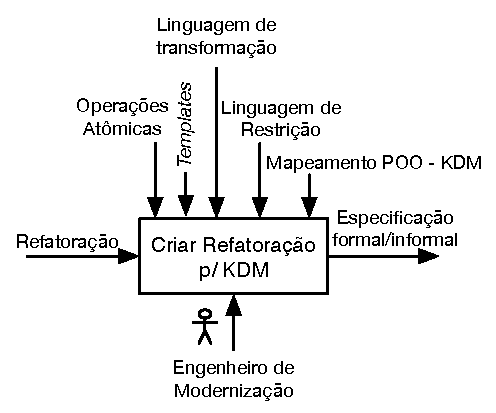
\includegraphics{figures/novoMacroAbordagemKDMRefactoring2.pdf}}
\end{figure}
  
\end{frame}

\begin{frame}\frametitle{Primeiro Passo da Abordagem}
  
\begin{minipage}[b]{10.80cm}
 A abordagem possui seis passos:
\end{minipage}  

\begin{figure}[!ht]
 \centering
 \scalebox{0.45}{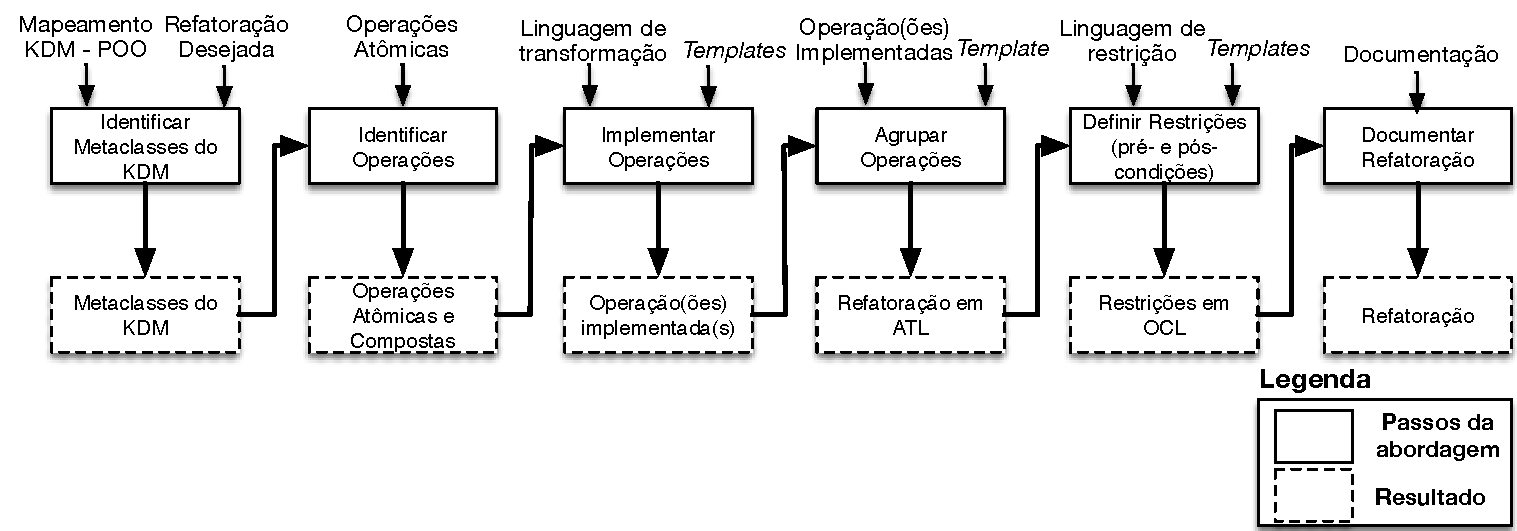
\includegraphics{figures/Abordagem_Criar_RefatoracaoFinal2.pdf}}
\end{figure}

  
  
\end{frame}

\begin{frame}\frametitle{Primeiro Passo da Abordagem}
  
\begin{minipage}[b]{10.80cm}
 A abordagem possui seis passos: Identificar Metaclasses do KDM.
\end{minipage}  

\begin{figure}[!ht]
 \centering
 \scalebox{0.45}{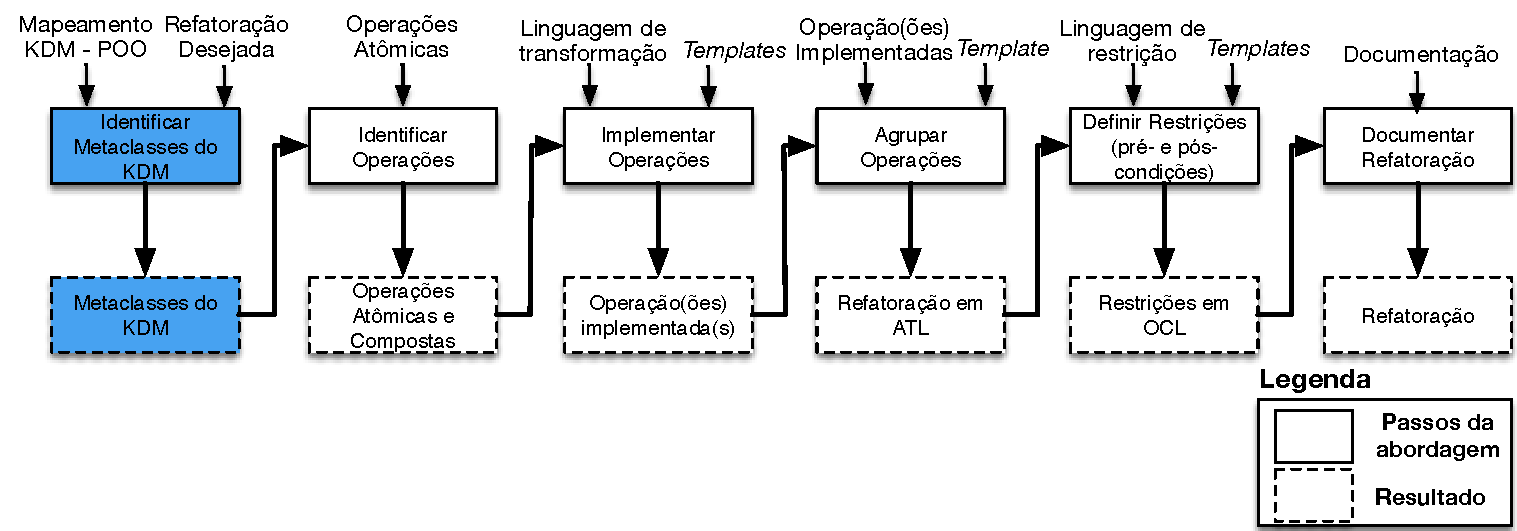
\includegraphics{figures/abordagemPasso1.pdf}}
\end{figure}
  
\end{frame}

%---------------------------vinicius stuffs







\begin{frame}[plain]
\frametitle{Identificar Metaclasses do KDM}

\begin{block}{\textbf{Engenheiro de Modernização}}
\begin{minipage}[b]{10.80cm}
 Deve identificar quais as metaclasses do KDM que representam os elementos do código-fonte.
\end{minipage}  
\end{block}



\tikzset{
  basic/.style  = {draw, text width=2cm, drop shadow, font=\sffamily, rectangle},
  root/.style   = {basic, rounded corners=2pt, thin, align=center,
                   fill=blue!15},
  level 2/.style = {basic, rounded corners=6pt, thin,align=center, fill=blue!25,
                   text width=8em},
  level 3/.style = {basic, thin, align=center, fill=blue!8.5, text width=4cm}
}

\begin{columns}
  \begin{column}{0.4\textwidth}

    \begin{tikzpicture}[
      level 1/.style={sibling distance=5mm},
      edge from parent/.style={->,draw},
      >=latex]

    % root of the the initial tree, level 1
    \node[root] {Refatoração}
    % The first level, as children of the initial tree
      child {node[level 2] (c2) {Engenheiro de M.}
      };

    % The second level, relatively positioned nodes
    \begin{scope}[every node/.style={level 3}]

    \node [below of = c2, xshift=40pt] (c21) {Mapeamento KDM e POO};
    \node [below of = c21] (c22) {Metaclasses do KDM};
    

    \end{scope}

    \foreach \value in {1,...,2}
      \draw[->] (c2.195) |- (c2\value.west);
    \end{tikzpicture}

  \end{column}
  \begin{column}{0.4\textwidth}
    
    
    \begin{itemize}
        \item Mapeamento entre KDM e POO
    \end{itemize}
    
\begin{table}[h]
\centering
\scriptsize
\label{tab:meta_classes_pacoteCODE}
\begin{tabular}{|l|l|}
\hline
Código-Fonte & Metaclasses do KDM \\ \hline
\multicolumn{1}{|c|}{Classe}                   & \multicolumn{1}{|c|}{\texttt{ClassUnit}}           \\ \hline
\multicolumn{1}{|c|}{Interface}                & \multicolumn{1}{|c|}{\texttt{InterfaceUnit}}       \\ \hline
\multicolumn{1}{|c|}{Método}                   & \multicolumn{1}{|c|}{\texttt{MethodUnit}}          \\ \hline
\multicolumn{1}{|c|}{Atributo}                 & \multicolumn{1}{|c|}{\texttt{StorableUnit}}        \\ \hline
\multicolumn{1}{|c|}{Variável Local}           & \multicolumn{1}{|c|}{\texttt{MemberUnit}}          \\ \hline
\multicolumn{1}{|c|}{Parâmetro}                & \multicolumn{1}{|c|}{\texttt{ParameterUnit}}       \\ \hline
\multicolumn{1}{|c|}{Associação}               & \multicolumn{1}{|c|}{\texttt{KDMRelationShip}}     \\ \hline
\end{tabular}
\end{table}

  \end{column}

\end{columns}

\end{frame}

\begin{frame}\frametitle{Segundo Passo da Abordagem}
  
\begin{minipage}[b]{10.80cm}
 A abordagem possui seis passos: Identificar Operações.
\end{minipage}  

\begin{figure}[!ht]
 \centering
 \scalebox{0.45}{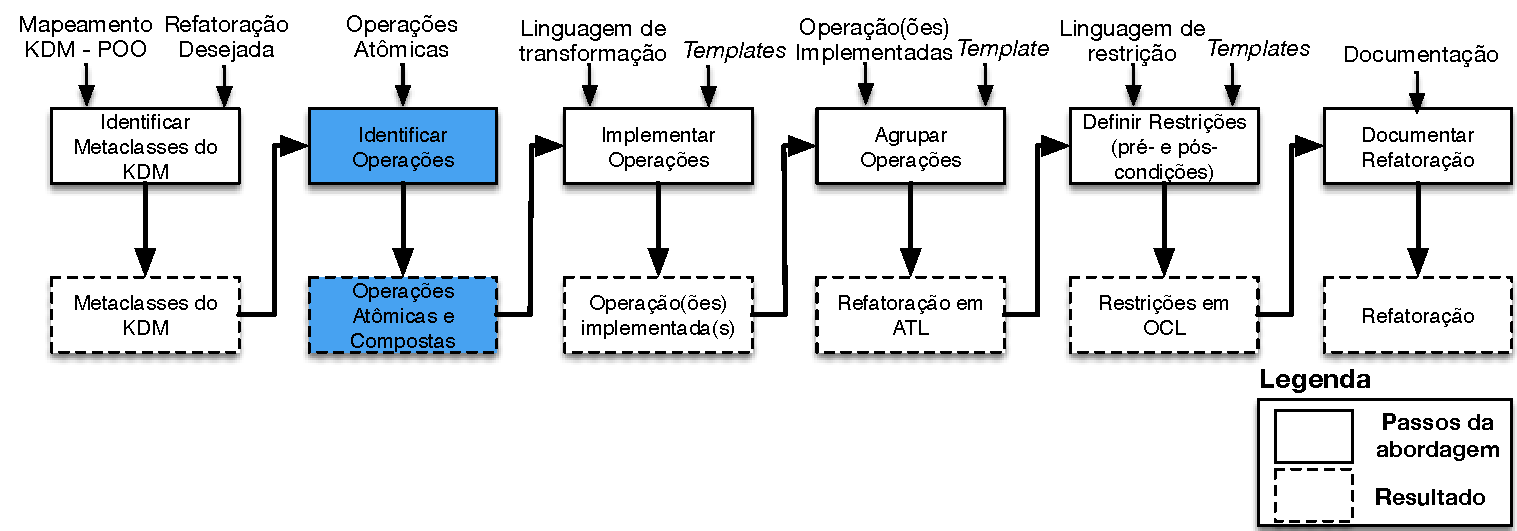
\includegraphics{figures/abordagemPasso2.pdf}}
\end{figure}
  
\end{frame}

\begin{frame}[plain]
\frametitle{Identificar Operações}

\begin{block}{\textbf{Engenheiro de Modernização}}
\begin{minipage}[b]{10.80cm}
 Deve identificar quais operações atômicas (add, delete e change) são utilizadas para criar a refatoração.
\end{minipage}
\end{block}
\tikzset{
  basic/.style  = {draw, text width=2cm, drop shadow, font=\sffamily, rectangle},
  root/.style   = {basic, rounded corners=2pt, thin, align=center,
                   fill=blue!15},
  level 2/.style = {basic, rounded corners=6pt, thin,align=center, fill=blue!25,
                   text width=8em},
  level 3/.style = {basic, thin, align=center, fill=blue!8.5, text width=4cm}
}

\begin{columns}
  \begin{column}{0.4\textwidth}

    \begin{tikzpicture}[
      level 1/.style={sibling distance=5mm},
      edge from parent/.style={->,draw},
      >=latex]

    % root of the the initial tree, level 1
    \node[root] {Operações Atômicas}
    % The first level, as children of the initial tree
      child {node[level 2] (c2) {Engenheiro de M.}
      };

    % The second level, relatively positioned nodes
    \begin{scope}[every node/.style={level 3}]

    \node [below of = c2, xshift=40pt] (c21) {Operação ADD};
    \node [below of = c21] (c22) {Operação DELETE};
    \node [below of = c22] (c23) {Operação CHANGE};
    

    \end{scope}

    \foreach \value in {1,...,3}
      \draw[->] (c2.195) |- (c2\value.west);
    \end{tikzpicture}

  \end{column}
  \begin{column}{0.4\textwidth}
    \begin{itemize}
        \item Identificar operações
    \end{itemize}
    \begin{figure}[!ht]
 \centering
 \scalebox{0.4}{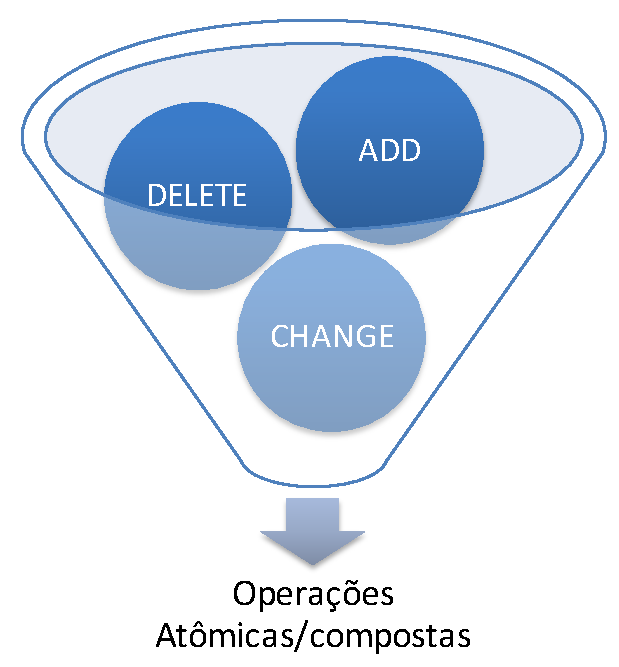
\includegraphics{figures/mixer.pdf}}
\end{figure}
    

  \end{column}

\end{columns}



\end{frame}



\begin{frame}\frametitle{Terceiro Passo da Abordagem}
  
\begin{minipage}[b]{10.80cm}
 A abordagem possui seis passos: Implementar Operações.
\end{minipage}  

\begin{figure}[!ht]
 \centering
 \scalebox{0.45}{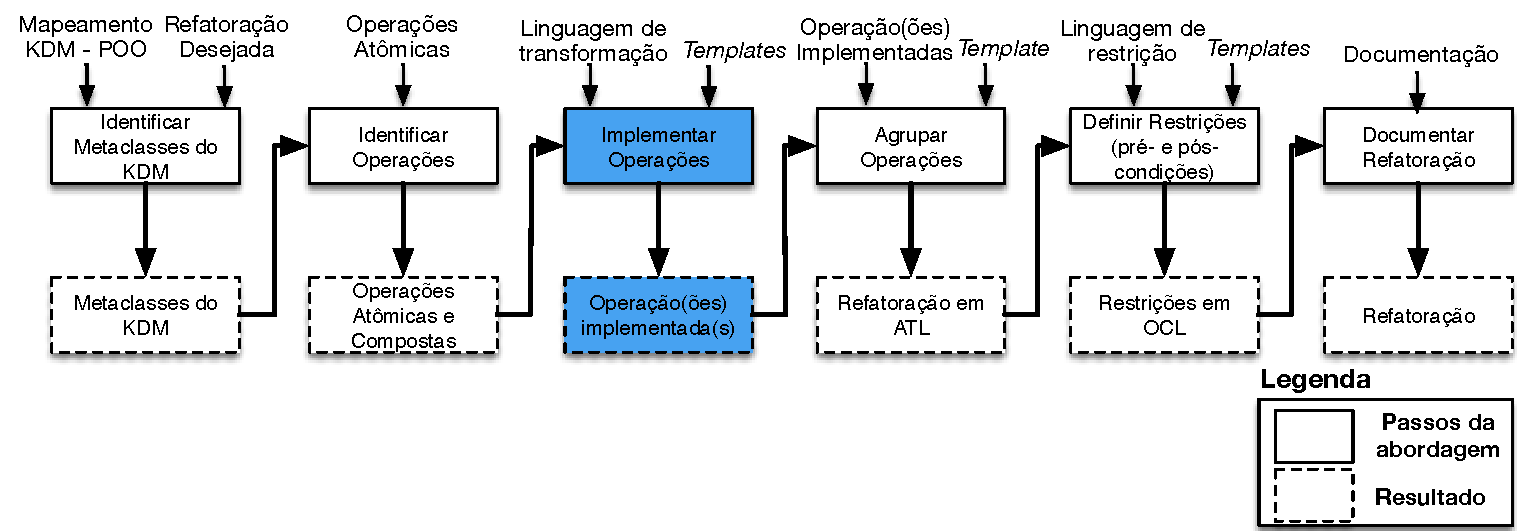
\includegraphics{figures/abordagemPasso3.pdf}}
\end{figure}
  
\end{frame}



\begin{frame}[plain]
\frametitle{Implementar Operações}

\begin{block}{\textbf{Engenheiro de Modernização}}
\begin{minipage}[b]{10.80cm}
 O engenheiro de modernização deve implementar as operações atômicas.
\end{minipage}
\end{block}
\tikzset{
  basic/.style  = {draw, text width=2cm, drop shadow, font=\sffamily, rectangle},
  root/.style   = {basic, rounded corners=2pt, thin, align=center,
                   fill=blue!15},
  level 2/.style = {basic, rounded corners=6pt, thin,align=center, fill=blue!25,
                   text width=8em},
  level 3/.style = {basic, thin, align=center, fill=blue!8.5, text width=4cm}
}

\begin{columns}
  \begin{column}{0.4\textwidth}

    \begin{tikzpicture}[
      level 1/.style={sibling distance=5mm},
      edge from parent/.style={->,draw},
      >=latex]

    % root of the the initial tree, level 1
    \node[root] {Templates - ATL}
    % The first level, as children of the initial tree
      child {node[level 2] (c2) {Engenheiro de M.}
      };

    % The second level, relatively positioned nodes
    \begin{scope}[every node/.style={level 3}]

    \node [below of = c2, xshift=40pt] (c21) {\textit{Template} ADD};
    \node [below of = c21] (c22) {\textit{Template} DELETE};
    \node [below of = c22] (c23) {\textit{Template} CHANGE};
    

    \end{scope}

    \foreach \value in {1,...,3}
      \draw[->] (c2.195) |- (c2\value.west);
    \end{tikzpicture}

  \end{column}
  \begin{column}{0.6\textwidth}
    \begin{itemize}
        \item Partes fixas: ATL
        \item Partes variantes:
            \begin{itemize}
                \item ArgX: <\# e \#> (\textit{Strings})
                \item ArgX: <\% e \%> (KDM)
                \item ArgX: <$@$ e $@$> (domínio)
            \end{itemize}
    \end{itemize}
    \begin{figure}[!ht]
 \centering
 \scalebox{0.3}{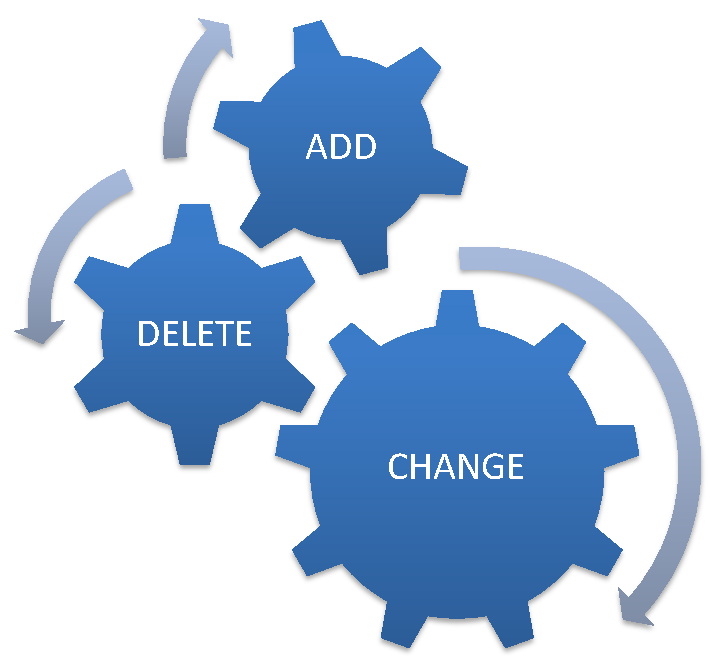
\includegraphics{figures/engrenagem.pdf}}
\end{figure}
    

  \end{column}

\end{columns}



\end{frame}


\begin{frame}\frametitle{Implementar Operações}
 
\begin{block}


\begin{minipage}[b]{10.80cm}
 Engenheiro de modernização deve substituir as partes variantes do \textit{template}.
\end{minipage}  

\end{block}

\begin{itemize}
    \item Tabelas são utilizadas para guiar a substituição.
\end{itemize}

\begin{figure}[!ht]
 \centering
 \scalebox{0.45}{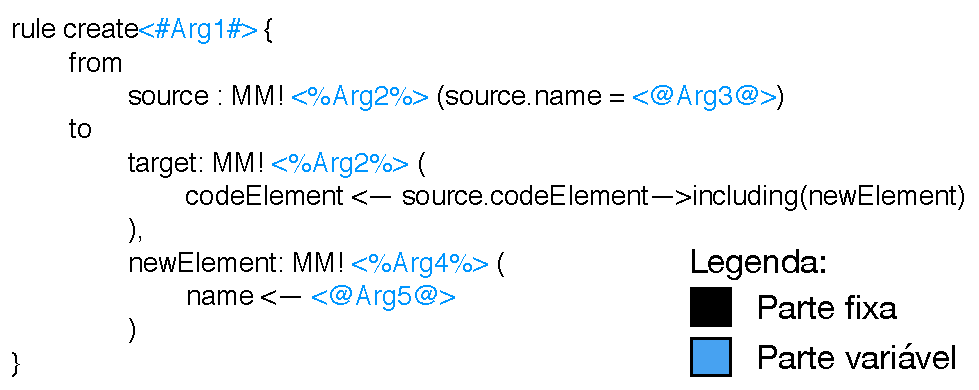
\includegraphics{figures/templateADD.pdf}}
\end{figure}
  
\end{frame}

\begin{frame}\frametitle{Implementar Operações}

\begin{figure}[!ht]
 \centering
 \scalebox{0.55}{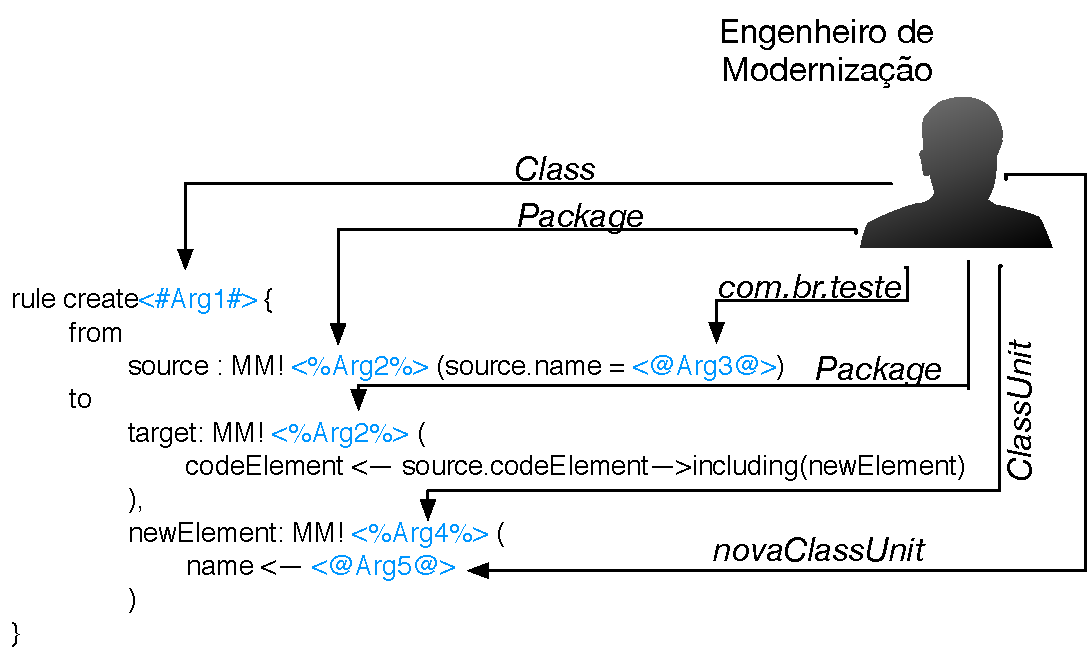
\includegraphics{figures/templateADDPreenchido.pdf}}
\end{figure}
  
\end{frame}



\begin{frame}\frametitle{Quarto Passo da Abordagem}
  
\begin{minipage}[b]{10.80cm}
 A abordagem possui seis passos: Agrupar Operações.
\end{minipage}  

\begin{figure}[!ht]
 \centering
 \scalebox{0.45}{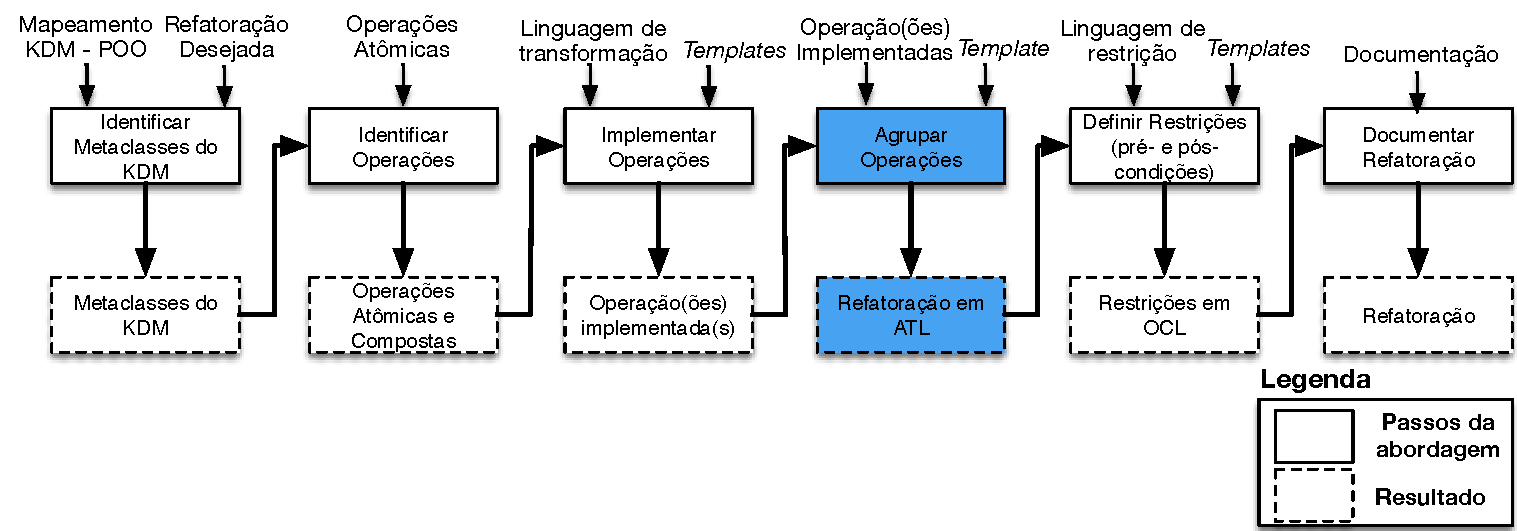
\includegraphics{figures/abordagemPasso4.pdf}}
\end{figure}
  
\end{frame}


\begin{frame}[plain]
\frametitle{Agrupar Operações}

\begin{block}{\textbf{Engenheiro de Modernização}}
\begin{minipage}[b]{10.80cm}
 O engenheiro de modernização deve agrupar as operações atômicas para formar a refatoração.
\end{minipage}
\end{block}
\tikzset{
  basic/.style  = {draw, text width=2cm, drop shadow, font=\sffamily, rectangle},
  root/.style   = {basic, rounded corners=2pt, thin, align=center,
                   fill=blue!15},
  level 2/.style = {basic, rounded corners=6pt, thin,align=center, fill=blue!25,
                   text width=8em},
  level 3/.style = {basic, thin, align=center, fill=blue!8.5, text width=4cm}
}

\begin{columns}
  \begin{column}{0.4\textwidth}

    \begin{tikzpicture}[
      level 1/.style={sibling distance=5mm},
      edge from parent/.style={->,draw},
      >=latex]

    % root of the the initial tree, level 1
    \node[root] {Operações Implementadas}
    % The first level, as children of the initial tree
      child {node[level 2] (c2) {Engenheiro de M.}
      };

    % The second level, relatively positioned nodes
    \begin{scope}[every node/.style={level 3}]

    \node [below of = c2, xshift=40pt] (c21) {\textit{Templates} ADD, DELETE e CHANGE};
    \node [below of = c21] (c22) {\textit{Template} guia};
    

    \end{scope}

    \foreach \value in {1,...,2}
      \draw[->] (c2.195) |- (c2\value.west);
    \end{tikzpicture}

  \end{column}
  \begin{column}{0.6\textwidth}
    \begin{itemize}
        \item Template para guiar o E.M
    \end{itemize}
    \begin{figure}[!ht]
 \centering
 \scalebox{0.4}{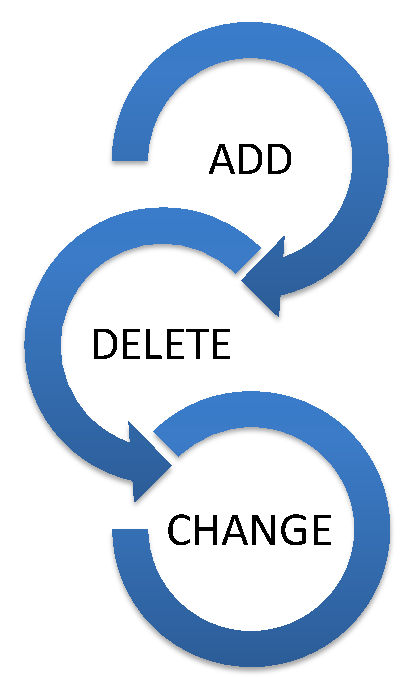
\includegraphics{figures/agrupar.pdf}}
\end{figure}
    

  \end{column}

\end{columns}



\end{frame}

\begin{frame}[plain]
\frametitle{Agrupar Operações}

\begin{block}{\textbf{Engenheiro de Modernização}}
\begin{minipage}[b]{10.80cm}
 O engenheiro de modernização deve agrupar as operações atômicas para formar a refatoração.
\end{minipage}
\end{block}
\tikzset{
  basic/.style  = {draw, text width=2cm, drop shadow, font=\sffamily, rectangle},
  root/.style   = {basic, rounded corners=2pt, thin, align=center,
                   fill=blue!15},
  level 2/.style = {basic, rounded corners=6pt, thin,align=center, fill=blue!25,
                   text width=8em},
  level 3/.style = {basic, thin, align=center, fill=blue!8.5, text width=4cm}
}

\begin{columns}
  \begin{column}{0.4\textwidth}

    \begin{tikzpicture}[
      level 1/.style={sibling distance=5mm},
      edge from parent/.style={->,draw},
      >=latex]

    % root of the the initial tree, level 1
    \node[root] {Operações Implementadas}
    % The first level, as children of the initial tree
      child {node[level 2] (c2) {Engenheiro de M.}
      };

    % The second level, relatively positioned nodes
    \begin{scope}[every node/.style={level 3}]

    \node [below of = c2, xshift=40pt] (c21) {\textit{Templates} ADD, DELETE e CHANGE};
    \node [below of = c21] (c22) {\textit{Template} guia};
    

    \end{scope}

    \foreach \value in {1,...,2}
      \draw[->] (c2.195) |- (c2\value.west);
    \end{tikzpicture}

  \end{column}
  \begin{column}{0.85\textwidth}
    \begin{itemize}
        \item Template para guiar o E.M
    \end{itemize}
    \begin{figure}[!ht]
 \centering
 \scalebox{0.4}{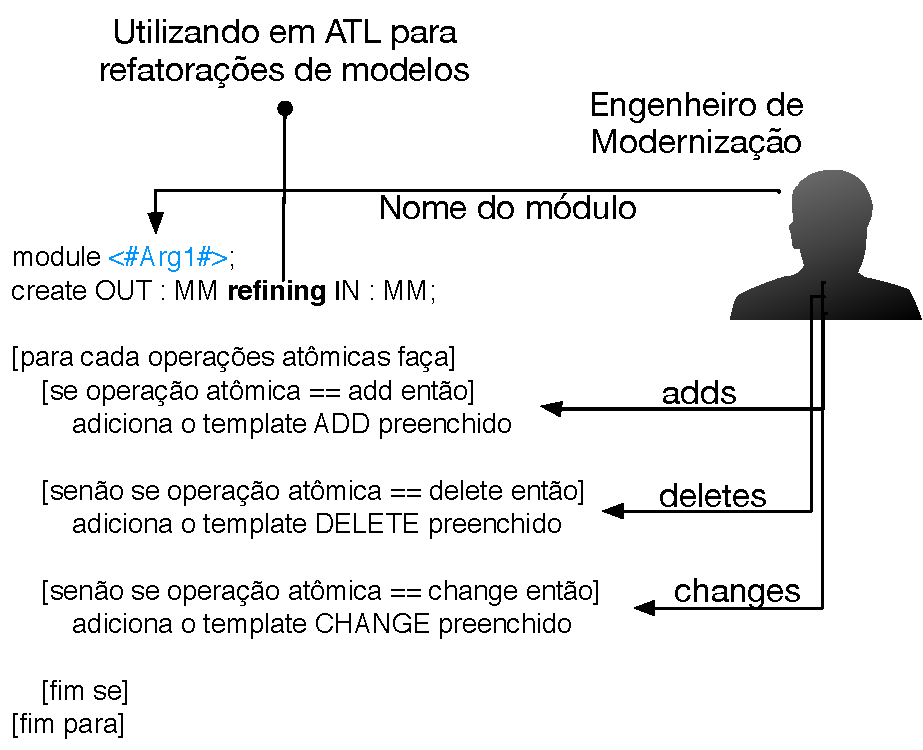
\includegraphics{figures/agrupar1.pdf}}
\end{figure}
    

  \end{column}

\end{columns}

\end{frame}


\begin{frame}\frametitle{Quinto Passo da Abordagem}
  
\begin{minipage}[b]{10.80cm}
 A abordagem possui seis passos: Definir Restrições (pré- e pós-condições).
\end{minipage}  

\begin{figure}[!ht]
 \centering
 \scalebox{0.45}{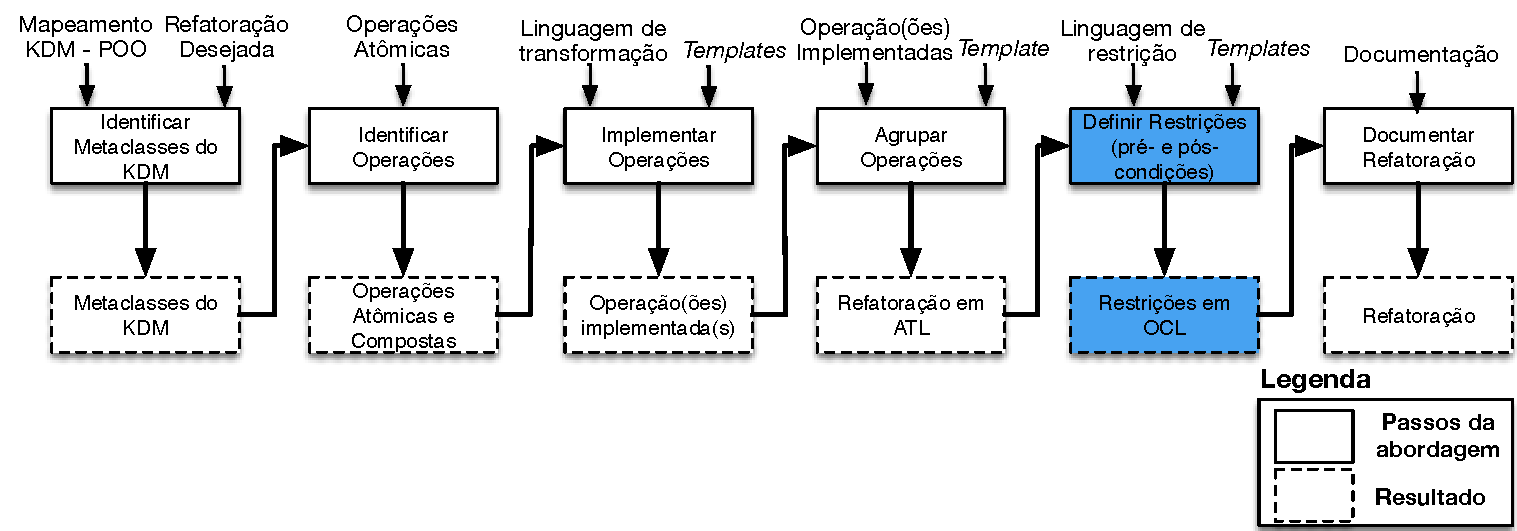
\includegraphics{figures/abordagemPasso5.pdf}}
\end{figure}
  
\end{frame}


\begin{frame}[plain]
\frametitle{Definir Restrições (pré- e pós-condições)}

\begin{block}{\textbf{Engenheiro de Modernização}}
\begin{minipage}[b]{10.80cm}
 O engenheiro de modernização deve implementar as restrições.
\end{minipage}
\end{block}
\tikzset{
  basic/.style  = {draw, text width=2cm, drop shadow, font=\sffamily, rectangle},
  root/.style   = {basic, rounded corners=2pt, thin, align=center,
                   fill=blue!15},
  level 2/.style = {basic, rounded corners=6pt, thin,align=center, fill=blue!25,
                   text width=8em},
  level 3/.style = {basic, thin, align=center, fill=blue!8.5, text width=4cm}
}

\begin{columns}
  \begin{column}{0.4\textwidth}

    \begin{tikzpicture}[
      level 1/.style={sibling distance=5mm},
      edge from parent/.style={->,draw},
      >=latex]

    % root of the the initial tree, level 1
    \node[root] {Templates - OCL}
    % The first level, as children of the initial tree
      child {node[level 2] (c2) {Engenheiro de M.}
      };

    % The second level, relatively positioned nodes
    \begin{scope}[every node/.style={level 3}]

    \node [below of = c2, xshift=40pt] (c21) {\textit{Templates} pré};
    \node [below of = c21] (c22) {\textit{Templates} pós};
    

    \end{scope}

    \foreach \value in {1,...,2}
      \draw[->] (c2.195) |- (c2\value.west);
    \end{tikzpicture}

  \end{column}
  \begin{column}{0.85\textwidth}
    \begin{itemize}
        \item Templates para guiar o E.M -> Pré e Pós
    \end{itemize}
    \begin{figure}[!ht]
 \centering
 \scalebox{0.4}{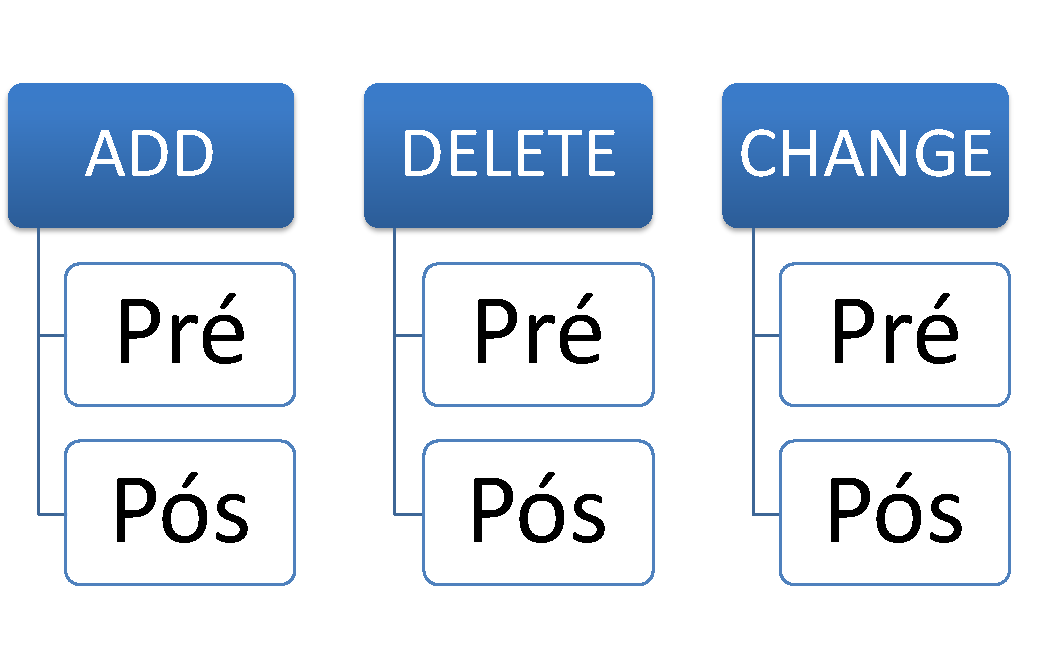
\includegraphics{figures/restricoesOCLSlide.pdf}}
\end{figure}
    

  \end{column}

\end{columns}

\end{frame}




\section{SRM: Um metamodelo para promover o reúso das refatorações para o KDM}
\frame{\tableofcontents[currentsection]}

\begin{frame}[t]\frametitle{Steps of the Proposed Ranking Method}

The proposed decision ranking method encompasses \textbf{seven steps}: 

\vspace{.3cm}

\begin{columns}
  \begin{column}{0.5\textwidth}
\tikz[baseline]{
            \node[fill=blue!20,anchor=base] (t1)
            {
            
            \begin{minipage}[b]{7cm} 
            \structure{\ding{202}} Segmentation and Identification of QAs; 
            \newline
            \structure{\ding{203}} Fixation of Acceptable Ranges for QAs;
            \newline
            \structure{\ding{204}} Normalization; 
            \newline
            \structure{\ding{205}} Creation of Desirability Curves for QAs; 
            \end{minipage}
              
            % \end{itemize}
            };
        }

        \tikz[baseline]{
            \node[fill=red!20,anchor=base] (t2)
            {
            
            \begin{minipage}[b]{7cm} 
            \structure{\ding{206}} Determination of the Weights of QAs; 
            \newline
            \structure{\ding{207}} Computation of Cumulative Scores; and
            \newline
            \structure{\ding{208}} Selection of the Design Decision.
            \end{minipage}
            };
        }
  \end{column}
  \begin{column}{0.5\textwidth} 
      \flushright
    % \begin{description}
      % \item Fine \color{white}~~~~~~~~~~~~~    
      \tikz\node [fill=blue!20,draw,circle] (n1) {Fine};
    % \end{description}
    % \begin{description}
      % \item \small Way too complex \color{white}\normalsize  
      \tikz\node [fill=red!20, below of=n1, draw,circle] (n2) {Hard};
    % \end{description}
  \end{column}
\end{columns}

\end{frame}

\begin{frame}\frametitle{Taking a Look at the Post-Questionnaire (1)}
  % \begin{figure}[t]
  %  \center
  %  \scalebox{0.397}{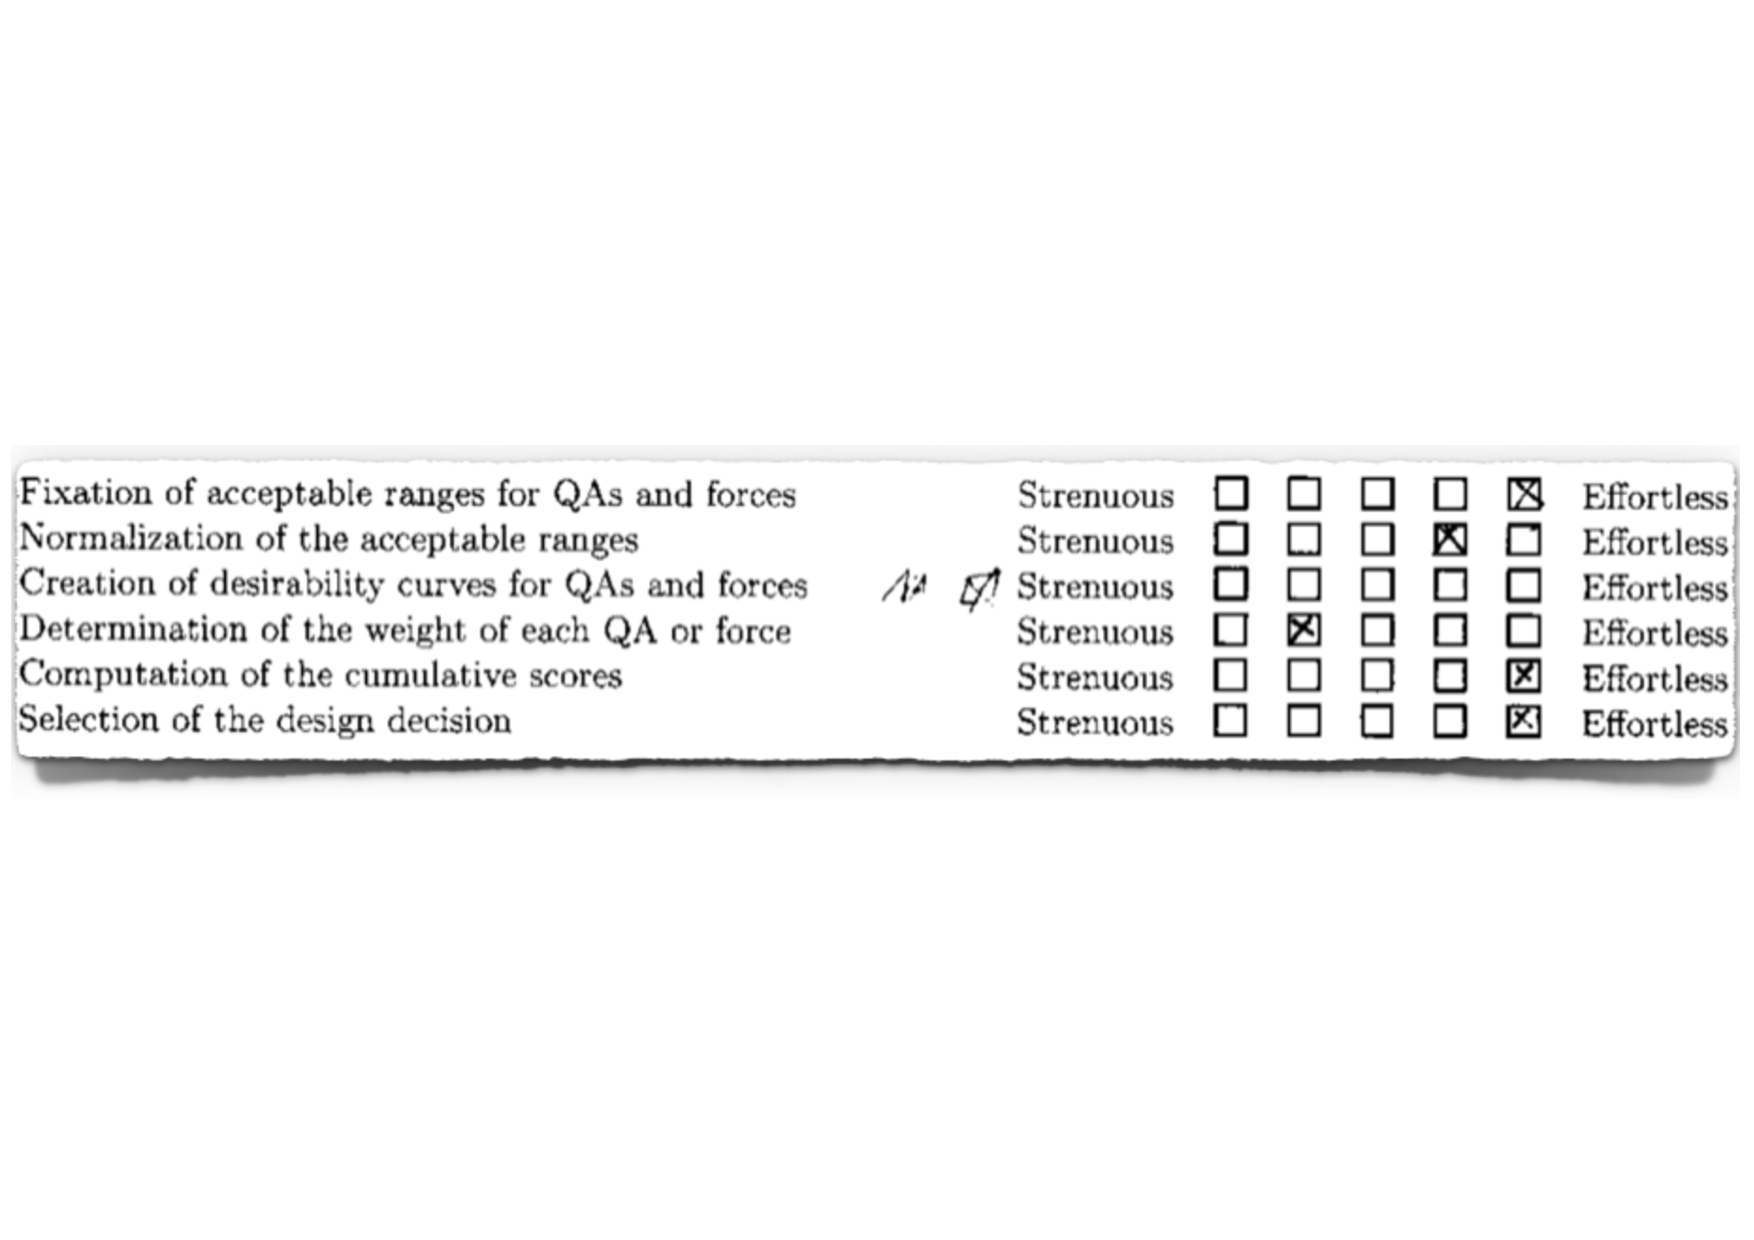
\includegraphics{questionnaire_part_1.pdf}}
  % \end{figure}  

  % \begin{tikzpicture}[font=\small]
  %   \foreach \line in {1,2} {
  %       \begin{scope}[yshift=-\line cm]
  %           \foreach \letter/\position in {\color{white}A/1, B/2, C/3, D/4, E/5} { 
  %               \node at (0,0) {\normalsize\textbf{\line}};
  %               \node[draw,rectangle,inner sep=1pt] at ({\position * 0.5},0) {\letter};
  %           }
  %       \end{scope}
  %   }
  % \end{tikzpicture}

  \begin{minipage}{10.8cm} 
  \structure{1.1 What do you think about the following steps of the decision ranking method in terms of the effort
        required to carry them out?}
  \end{minipage}

  \begin{description}
    \item Fixation of acceptable ranges for QAs/forces \tiny(Step~\structure{\ding{203}})\normalsize
    \begin{flushright}
      \begin{tikzpicture}[font=\small]
        \begin{scope}[yshift=-1 cm]
            \foreach \letter/\position in {\color{white}A/1, \color{white}B/2, \color{white}C/3, \color{white}D/4, \ding{51}/5} { 
                \node at (0,0) {\tiny Strenuous~~~~~~~~};
                \node[draw,rectangle,inner sep=1pt] at ({\position * 0.5},0) {\letter};
                \node at (3.4,0) {\tiny Effortless};
            } 
        \end{scope}
  \end{tikzpicture}
    \end{flushright}
      
    \item Normalization of the acceptable ranges \tiny(Step~\structure{\ding{204}})\normalsize 
    \begin{flushright}
      \begin{tikzpicture}[font=\small]
        \begin{scope}[yshift=-1 cm]
            \foreach \letter/\position in {\color{white}A/1, \color{white}B/2, \color{white}C/3, \ding{51}/4, \color{white}E/5} { 
                \node at (0,0) {\tiny Strenuous~~~~~~~~};
                \node[draw,rectangle,inner sep=1pt] at ({\position * 0.5},0) {\letter};
                \node at (3.4,0) {\tiny Effortless};
            } 
        \end{scope}
  \end{tikzpicture}
    \end{flushright}

    \item Creation of desirability ranges for QAs/forces \tiny(Step~\structure{\ding{205}})\normalsize
    \begin{flushright}
      \begin{tikzpicture}[font=\small]
        \begin{scope}[yshift=-1 cm]
            \foreach \letter/\position in {\color{white}A/1, \color{white}B/2, \color{white}C/3, \color{white}D/4, \color{white}E/5} { 
                \node at (0,0) {\tiny Strenuous~~~~~~~~};
                \node[draw,rectangle,inner sep=1pt] at ({\position * 0.5},0) {\letter};
                \node at (3.4,0) {\tiny Effortless};
            } 
        \end{scope}
  \end{tikzpicture}
  \end{flushright}
          
  \end{description}
  
\end{frame}

\begin{frame}\frametitle{Taking a Look at the Post-Questionnaire (2)}

  \begin{minipage}{10.8cm} 
  \structure{1.1 What do you think about the following steps of the decision ranking method in terms of the effort
        required to carry them out?}
  \end{minipage}

    \begin{description}
      
      \item Determination of the weight of each QA/force \tiny(Step~\structure{\ding{206}})\normalsize
      \begin{flushright}
        \begin{tikzpicture}[font=\small]
        \begin{scope}[yshift=-1 cm]
            \foreach \letter/\position in {\color{white}A/1, \ding{51}/2, \color{white}C/3, \color{white}D/4, \color{white}E/5} { 
                \node at (0,0) {\tiny Strenuous~~~~~~~~};
                \node[draw,rectangle,inner sep=1pt] at ({\position * 0.5},0) {\letter};
                \node at (3.4,0) {\tiny Effortless};
            } 
        \end{scope}
  \end{tikzpicture}
      \end{flushright}
          
    \item Computation of cumulative scores \tiny(Step~\structure{\ding{207}})\normalsize
    \begin{flushright}
                \begin{tikzpicture}[font=\small]
        \begin{scope}[yshift=-1 cm]
            \foreach \letter/\position in {\color{white}A/1, \color{white}B/2, \color{white}C/3, \color{white}D/4, \ding{51}/5} { 
                \node at (0,0) {\tiny Strenuous~~~~~~~~};
                \node[draw,rectangle,inner sep=1pt] at ({\position * 0.5},0) {\letter};
                \node at (3.4,0) {\tiny Effortless};
            } 
        \end{scope}
  \end{tikzpicture}
      
    \end{flushright}
    \item Selection of the design decision \tiny(Step~\structure{\ding{208}})\normalsize
    \begin{flushright}
                \begin{tikzpicture}[font=\small]
        \begin{scope}[yshift=-1 cm]
            \foreach \letter/\position in {\color{white}A/1, \color{white}B/2, \color{white}C/3, \color{white}D/4, \ding{51}/5} { 
                \node at (0,0) {\tiny Strenuous~~~~~~~~};
                \node[draw,rectangle,inner sep=1pt] at ({\position * 0.5},0) {\letter};
                \node at (3.4,0) {\tiny Effortless};
            } 
        \end{scope}
  \end{tikzpicture}      
    \end{flushright}

  \end{description}
  
\end{frame}

\begin{frame}\frametitle{Taking a Look at the Post-Questionnaire (3)}

  \begin{minipage}{10.8cm} 
  \structure{1.2 How do you rate the overall effort required to carry out the decision ranking method?}
  \end{minipage}
  \begin{description}
    \item \color{white}AAAA\color{black}
    \begin{flushright}
                \begin{tikzpicture}[font=\small]
        \begin{scope}[yshift=-1 cm]
            \foreach \letter/\position in {\color{white}A/1, \color{white}B/2, \ding{51}/3, \color{white}D/4, \color{white}D/5} { 
                \node at (0,0) {\tiny Strenuous~~~~~~~~};
                \node[draw,rectangle,inner sep=1pt] at ({\position * 0.5},0) {\letter};
                \node at (3.4,0) {\tiny Effortless};
            } 
        \end{scope}
  \end{tikzpicture}      
    \end{flushright}
  \end{description}

  \vspace{0.3cm}
  \begin{minipage}{10.8cm} 
  \structure{1.3 The results made it easy for me to better evaluate the trade-offs among the decisions and their architectural implications?}
  \end{minipage}
  \begin{description}
    \item \color{white}AAAA\color{black}
    \begin{flushright}
                \begin{tikzpicture}[font=\small]
        \begin{scope}[yshift=-1 cm]
            \foreach \letter/\position in {\color{white}A/1, \color{white}B/2, \ding{51}/3, \color{white}D/4, \color{white}D/5} { 
                \node at (0,0) {\tiny Strongly agree~~~~~~~~~~~~};
                \node[draw,rectangle,inner sep=1pt] at ({\position * 0.5},0) {\letter};
                \node at (3.4,0) {\tiny ~~~~~Strongly disagree};
            } 
        \end{scope}
  \end{tikzpicture}      
    \end{flushright}
  \end{description}

\end{frame}

\begin{frame}\frametitle{Taking a Look at the Post-Questionnaire (4)}
  \framesubtitle{Free-form Questions}
  \begin{minipage}{10.8cm} 
  \structure{2.1 What are the major strengths of the decisions ranking method?}
  \end{minipage}

  \textbf{R.} \ding{125}Structured way to identify relative priorities of forces.\ding{126}

  \vspace{.3cm}
  \begin{minipage}{10.8cm} 
  \structure{2.2 What are the major drawbacks of the decision ranking method?}
  \end{minipage}
  \begin{minipage}{10.80cm}
    \textbf{R.} \ding{125}[...] coming up with \emph{HE decisions} is not as trivial and 
    already requires that the weight of the forces is known [...]\ding{126}
    \vspace{0.2cm}
    \par \ding{125}
    I am wondering if stakeholders could come up with HE decisions 
    why do they need to rank forces in the first place?\ding{126} 
    \vspace{0.2cm}
    \par \ding{125}
    [...] this method requires more effort if more than three forces 
    need to be considered. It seems that it does not scale that well.\ding{126}

  \end{minipage}
\end{frame}


\begin{frame}\frametitle{Taking a Look at the Post-Questionnaire (5)}
  \framesubtitle{Free-form Questions}
  \begin{minipage}{10.8cm} 
  \structure{2.3 Do you have any comments regarding the practical difficulties of 
  applying the decision ranking method?}
  \end{minipage}

  \begin{minipage}{10.8cm}
    \vspace{.15cm}
    \textbf{R.} \ding{125}[...] it seems as if this method produces the best result if it is performed by a group of people 
  (of the same stakeholder group)\newline 
  \par [...] but we couldn't try this scenario in the pilot.\ding{126}
  \end{minipage}

\end{frame}

\section{A ferramenta KDM-RE} 
\label{sec:where_to_go_from_here_}
\frame{\tableofcontents[currentsection]}


% \definecolor{myblue}{RGB}{83,121,200}

\tikzset{
myshape/.style={
  shape=signal,
  fill=blue!63,
  minimum height=1.5cm,
  minimum width=1.5cm,
  text=white,
  signal pointer angle=130,
  signal to=east,
  signal from=west,
  rotate=-90,
  transform shape
  },
mytext/.style={
  draw=blue!63,
  text width=7cm,
  minimum height=1.15cm,
  thick,
  outer sep=0pt
  }  
}
\newcounter{tmp}
\newcommand\MyDesc[3][]{
\stepcounter{tmp}%
\node[myshape,#1] (desc\thetmp) {};
\node[font=\color{white}] at (desc\thetmp) {#2};
\node[mytext,anchor=north west] at (desc\thetmp.north west) 
  {%
    \parbox[t]{2em}{\hfill$\bullet$\hfill\null}%
    \parbox[t]{\dimexpr\linewidth-2em\relax}{#3}%
  };
}

\begin{frame}[plain]\frametitle{Interpreting the Results: The HE Seems to be the Problem\ldots}
  
\setbeamercolor{footnote mark}{fg=white}

Characterization schema: commonalities and variabilities
\vspace{.2cm}

\begin{tikzpicture}[]

  \MyDesc{\tiny Description}{Step: \structure{\ding{202}}}

  \MyDesc[below = 1.5cm of desc1.north]{\tiny Importance}{Steps: \structure{\ding{203}}, \structure{\ding{204}}}

  \MyDesc[below = 1.5cm of desc2.north]{\tiny Fitness{\footnote{$^1$ Fulfillment.}}}{Steps: \structure{\ding{205}}, \structure{\ding{206}}}

  \uncover<2-3>{
  \MyDesc[below = 1.5cm of desc2.north]{\tiny Fitness$^1$}{Steps: \structure{\ding{205}}, \textbf{\color{red}X}}
  }

  \uncover<3>{
  \MyDesc[below = 1.5cm of desc3.north]{\tiny Uncertainty}{Steps: 
  so far, none.}
  }
\end{tikzpicture}
\end{frame}

% \begin{frame}\frametitle{}

% \begin{minipage}{10.8cm}
% At this point, we want something that \textbf{avoids the selection of a worse alternative} and, at the same time, it is \textbf{easy to use}. 
% \end{minipage}

% \begin{itemize}
%   \item todo
%   \item todo
%   \item todo
%   \item todo  
% \end{itemize}
% \end{frame}

\section{Avaliação}
\label{sec:wrapping_up}

\begin{frame}\frametitle{Concluding Remarks\ldots}
  \begin{itemize}
    \begin{minipage}{9.8cm}\item Provides a systematic way to ponder about decisions;\vspace{0.2cm}\end{minipage}
    \begin{minipage}{9.8cm}\item \textbf{Quantitative overview} of how each decision performs on 
    important QAs/forces;\vspace{0.2cm}\end{minipage}
    \begin{minipage}{9.8cm}\item \textbf{Downside:} highly \textbf{``mathy''}, \textbf{cumbersome};\vspace{0.2cm}\end{minipage}
    \begin{minipage}{9.8cm}\item \textbf{Future:} 
    Replace the HE method and carry out an \textbf{empirical study} to evaluate how well the ranking method works for graduate students.\vspace{0.2cm}\end{minipage} 
  \end{itemize}
\end{frame}

\section{Conclusões}
\subsection{Contribuições, Limitações, Trabalhos Futuros e Publicações}


\begin{frame}[plain,c]\frametitle{}
\begin{center}
% Well that brings me to the end of the presentation. 
% Thank you for your attention.
\Huge
``What a Long, Strange Trip It's Been''\footnote{
  \textbf{\tiny What a Long, Strange Trip It's Been}, by Grateful Dead, is arguably one of the most famous lines in rock and roll. This snippet has entitled several books and articles since the song's release. Since it evokes a lifespan of constant changes, I believe it fits perfectly to describe my stay here.
  } \\
  \pause
\Huge \textbf{Thank you!}
\smiley
\end{center}
  
\end{frame}

\begin{frame}\frametitle{Bibliografia}
  % estilo da bibliografia
  \bibliographystyle{abbrv}
  % chamando o arquivo refs.bib
  \bibliography{references}
\end{frame}

% \frame[plain,c]{
% \begin{center}
% % Well that brings me to the end of the presentation. 
% % Thank you for your attention.
% \Huge \textbf{Thank you!}
% \smiley
% \end{center}
% }

\end{document}
